\documentclass{article}
\usepackage[utf8]{inputenc}
\usepackage{subcaption}
\usepackage{amsmath}
\usepackage{amssymb}
\usepackage{hyperref}
\usepackage{titlesec}
\usepackage{xcolor}
\usepackage{fancyhdr}
\usepackage{graphicx}
\usepackage{multirow}
\usepackage[rightcaption]{sidecap}
\usepackage{verbatim}
\usepackage[backend=bibtex]{biblatex}
\addbibresource{references.bib}

\usepackage [ a4paper , hmargin =1.2 in , bottom =1.5 in ] { geometry }
\hypersetup{
    colorlinks=true,
    linkcolor=blue,
    filecolor=magenta,      
    urlcolor=cyan,
}


% Add header and footer code here
% You may also add path to the images optionally
\pagestyle{fancy}
\fancyhf{}
\lhead{Transformation of R.V. and Multivariate Gaussian}
\rhead{Harshil Solanki}
\fancyfoot[C]{Page \thepage}
% preamble
\begin{document}
\title{
Transformation of R.V. \\
and \\
Multivariate Gaussian
}
\author{Harshil Solanki}
\date{}
\maketitle
% below line auto generates the table of contents
% thank me for your free 1 mark
\tableofcontents
\clearpage

%code of section 1, with lists
\section{Introduction}
In this article, we will study about the following topics of statistics:
\begin{itemize}
\item Transformation of random veriables
\item Multivariate Gaussian random variable
\end{itemize}
%code of section 2, make appr
%para
% \[\]
%para.....
% \begin{equation}
% \end{equation}
\section{Transformation of Random Variable}
Given any continuous r.v. $X$ with PDF $P_X(x)$ and given any function $g(X)$(defined on range of $X$) we intend to find PDF associated with the r.v. $Y = g(X)$.\\
Then by probability mass conservation,
\[
P(a<X<b) = P(g(a)<Y<g(b)) = \int_{g(a)}^{g(b)} Q(y)dy
\]
Using $y=g(x)$, we get the below relation upon simplification
\[
Q(y) = P(g^{-1}(y))\frac{g(d(g^{-1}(y)))}{dy}
\]
To handle monotonically decreasing $g(.)$ as well\footnote[1]{we could have used modulus operator but I wanted things to look more complicated},
\begin{equation}
    Q(y)=
    \begin{cases}
        +P(g^{-1}(y))\frac{g(d(g^{-1}(y)))}{dy} & \text{for $g(.)$ monotonically increasing}\\
        -P(g^{-1}(y))\frac{g(d(g^{-1}(y)))}{dy} & \text{for $g(.)$ monotonically increasing}
    \end{cases}
\end{equation}
For more information, refer \cite{ref1}

\begin{figure}[h!]
%     % code for subfigure, label them for using references
\begin{subfigure}[b]{0.5\textwidth}
    \centering
    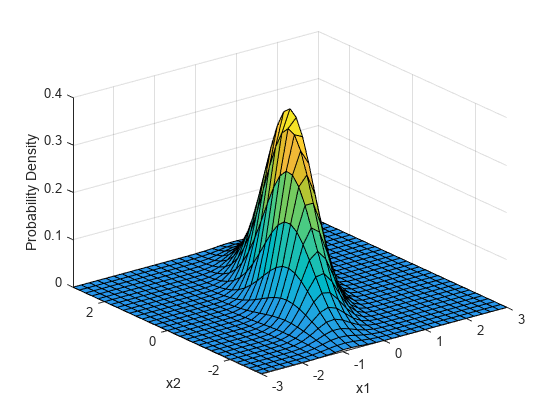
\includegraphics[width=\textwidth]{images/multivariate_gaussian.png}
    \caption[(a)]{Example 1}
    \label{fig:fig1}
\end{subfigure}
\begin{subfigure}[b]{0.5\textwidth}
    \centering
    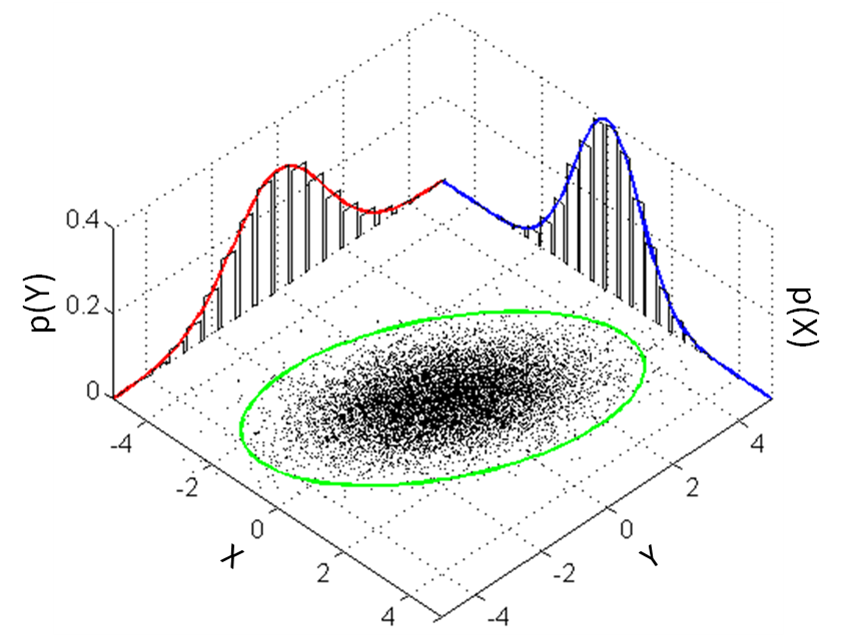
\includegraphics[width=\textwidth]{images/multivariate_normal.png}
    \caption[(a)]{Example 2}
    \label{fig:fig2}
\end{subfigure}
\end{figure}

%code for section 3
\section{Multi-variate Gaussian Disribution}
\subsection{Definition}
Let $X$ be a vector of random variables of dimension $D$.\\
A r.v. X has a joint PDF as multi-variate Gaussian distribution $\exists$ finite i.i.d. standard Gaussian r.v. $W_1, W_2,\dots W_n$ with $N>D$ such that
\[
X = AW + \mu
\]
Refer fig[\ref{fig:fig1}] and fig[\ref{fig:fig2}] for visual examples.This has many applications in machine learning, refer \cite{ref3} and \cite{ref2}

\subsection{A is diagonal}
In this case, the $X_i$ are independent. The standard deviation of distribution of $X_i$ is $A_{ii}$.
\subsection{A is non-singular square matrix}

Let's take µ = 0 for simplicity.\\
Similar to univariate case, where scaling was determined by $\left\lvert \frac{d(g^{-1}(y))}{dy}\right\rvert$, the scaling for multi-variate
case is determined by determinant of matrix of derivatives, Jacobian matrix.\\
Also, $W = A^{-1}X$, which is a linear transformation of vector $X$. $A^{-1}$ maps a hypercube to parallelepiped. If the vectors describing the hypercube are along cardinal axis, then the parallelepiped is described by vectors which are columns of $A^{-1}$.\\
We intend to find the volume of the parallelepiped formed due to this transformation.\\
{\bfseries Claim:} The volume of parallelepiped described by column vectors of matrix $A^{-1}$ is given by $det(A^{-1})$\\
{\bfseries Proof:} Addition of any scaled column of a matrix M to another column does not change the
determinant.\\
Therefore by Gram-Schmidt orthogonalization process the columns of $A^{-1}$ can be constructedto be orthogonal to each other, without changing the determinant. Then multiplying by an orthogonal matrix would rotate the orthogonal vectors(to align them with cardinal axis), and this
operation would not change the determinant as well. Now the result matrix is diagonal square
matrix and the volume of the parallelepiped described by the column vectors is given by product
of diagonal elements.\\
\\
From the above result, an infinitesimal volume $\delta^D$ after transformation becomes $\delta^D\cdot det(A^{-1})$.\\
\\
Let $C = A \cdot A^T$. Then $det(A)=\sqrt{det(C)}$. The above expression can be rewritten as
\begin{equation}
    P(X)=\frac{1}{(2\pi)^{D/2}}\cdot \frac{1}{\sqrt{det(C)}}\cdot exp(0.5\cdot X^T \cdot C^{-1}\cdot X)
\end{equation}

\begin{tabular}{|l|l||l|}
% ... fill up table
\hline
\multicolumn{3}{|c|}{Sample Values of bivariate normal distribution}\\
\hline
x&y&f(x,y)\\
\hline
0&0&1.6\\
0&1&0.096\\
$\sqrt{2}$&$\sqrt{2}$&0.02\\
\hline
\end{tabular}


% print the bibliography
\printbibliography
\end{document}